\chapter[Backtracking]
{Backtracking
  \label{chBcktrcking}}
\chaptermark{Backtracking}


\section{Introduction\label{BktrckIntro}}

Here is a collection of intros to try ease myself into the subject.



\rrsepline


\url{http://algorithms.tutorialhorizon.com/introduction-to-backtracking-programming/}

\rrheader{Introduction To Backtracking Programming}

\noindent{}\textbf{What is Backtracking Programming??}

Recursion is the key in backtracking programming. As the name suggests we
back­track to find the solution. We start with one possible move out of many
available moves and try to solve the problem if we are able to solve the
problem with the selected move then we will print the solution else we will
back­track and select some other move and try to solve it. If none if the
moves work out we will claim that there is no solution for the problem.

\noindent{}\textbf{Generalized Algorithm:}
\begin{lstlisting}[style=pseudostyle,numbers=none]
Pick a starting point.
while(Problem is not solved)
  For each path from the starting point.
    check if selected path is safe, if yes select it
                and make recursive call to rest of the problem
		If recursive calls returns true, then return true.
		else undo the current move and return false.
	End For
	If none of the move works out, return false, NO SOLUTON.
\end{lstlisting}


\rrsepline

Wikipedia: \url{https://en.wikipedia.org/wiki/Backtracking}

\textbf{Backtracking} is a general algorithm for finding all (or some)
solutions to some computational problems, notably constraint satisfaction
problems, that incrementally builds candidates to the solutions, and
abandons each partial candidate (``backtracks'') as soon as it determines
that the candidate cannot possibly be completed to a valid solution.

The classic textbook example of the use of backtracking is the eight queens
puzzle\footnote{\url{https://en.wikipedia.org/wiki/Eight\_queens\_puzzle}},
that asks for all arrangements of eight chess queens on a standard
chessboard so that no queen attacks any other. In the common backtracking
approach, the partial candidates are arrangements of $k$ queens in the first
$k$ rows of the board, all in different rows and columns. Any partial
solution that contains two mutually attacking queens can be abandoned.

Backtracking can be applied only for problems which admit the concept of a
``partial candidate solution'' and a relatively quick test of whether it can
possibly be completed to a valid solution. It is useless, for example, for
locating a given value in an unordered table. When it is applicable,
however, backtracking is often much faster than brute force enumeration of
all complete candidates, since it can eliminate a large number of candidates
with a single test.

Backtracking is an important tool for solving constraint satisfaction
problems, such as crosswords, verbal arithmetic, Sudoku, and many other
puzzles. It is often the most convenient (if not the most efficient)
technique for parsing, for the knapsack problem and other combinatorial
optimization problems. It is also the basis of the so-called logic
programming languages such as Icon, Planner and Prolog.

The term ``backtrack'' was coined by American mathematician D. H. Lehmer in
the 1950s. The pioneer string-processing language SNOBOL (1962) may have
been the first to provide a built-in general backtracking facility.

\rrheader{Description of the method}

The backtracking algorithm enumerates a set of \textbf{\emph{partial
    candidates}} that, in principle, could be \textbf{\emph{completed}} in
various ways to give all the possible solutions to the given problem. The
completion is done incrementally, by a sequence of \textbf{\emph{candidate
    extension}} steps.

Conceptually, the \emph{partial candidates} are represented as the
\textbf{\emph{nodes of a tree structure, the potential search tree}}. Each
\emph{partial candidate} is the \emph{parent of the candidates that differ
  from it by a \textbf{single extension step}}; the \textbf{leaves} of the
tree are the \textbf{partial candidates that cannot be extended any
  further}.

The backtracking algorithm traverses this search tree recursively, from the
root down, in depth-first order. At each node $c$, the algorithm checks
whether $c$ can be completed to a valid solution. If it cannot, the whole
sub-tree rooted at $c$ is skipped (pruned). Otherwise, the algorithm
\textbf{(1)} checks whether $c$ itself is a valid solution, and if so
reports it to the user; and \textbf{(2)} recursively enumerates all
sub-trees of $c$. The two tests and the children of each node are defined by
user-given procedures.

Therefore, the \textbf{actual search tree} that is traversed by the
algorithm is only a \textbf{part of the potential tree}. The total cost of
the algorithm is the number of nodes of the \textbf{actual tree} times
\textbf{the cost of obtaining and processing each node}. This fact should be
considered when \textbf{(1)} choosing the potential search tree and
\textbf{(2)} implementing the pruning test.

\rrheader{Pseudocode}

In order to apply backtracking to a specific class of problems, one must
provide the data $P$ for the particular instance of the problem that is to
be solved, and six procedural parameters, \ctt{root}, \ctt{reject},
\ctt{accept}, \ctt{first}, \ctt{next}, and \ctt{output}. These procedures
should take the instance data $P$ as a parameter and should do the
following:
\begin{enumerate}[label=\textbf{\arabic*.}]
\item \ctt{root(P)}: return the partial candidate at the root of the search
  tree.
\item \ctt{reject(P,c)}: return true only if the partial candidate $c$ is
  not worth completing. The \ctt{reject(P,c)} procedure should be a
  boolean-valued function that returns \texttt{true} only if it is certain
  that no possible extension of $c$ is a valid solution for $P$. If the
  procedure cannot reach a definite conclusion, it should return
  \texttt{false}.
\item \ctt{accept(P,c)}: return \texttt{true} if $c$ is a solution of $P$,
  and \texttt{false} otherwise.
\item \ctt{first(P,c)}: generate the first extension of candidate $c$.
\item \ctt{next(P,s)}: generate the next alternative extension of a
  candidate, after the extension $s$.
\item \ctt{output(P,c)}: use the solution $c$ of $P$, as appropriate to the
  application.
\end{enumerate}
The backtracking algorithm reduces the problem to the call
\ctt{bt(root(P))}, where \ctt{bt} is the following recursive procedure:
\begin{lstlisting}[style=pseudostyle,numbers=none]
procedure bt(c)
  if reject(P,c) then return
  if accept(P,c) then output(P,c)
  s := first(P,c)
  while s $\neq\Lambda$ do
    bt(s)
    s := next(P,s)
\end{lstlisting}

\rrblue{(I'm not quite sure how \ctt{next} works, but I think it might be
  like returning a sibling of $s$. This would make sense since we do
  depth-first order, then after this node $s$, we run the same algo on a
  sibling of $s$.  I'll find out later when I look at implementations.)}

\rrheader{Usage considerations}

The \ctt{reject(P,c)} procedure should be a boolean-valued function that
returns \texttt{true} only if it is certain that no possible extension of
$c$ is a valid solution for $P$. If the procedure cannot reach a definite
conclusion, it should return \texttt{false}. An incorrect \texttt{true}
result may cause the \ctt{bt} procedure to miss some valid solutions. The
procedure may assume that \ctt{reject(P,t)} returned \texttt{false} for
every ancestor $t$ of $c$ in the search tree \rrblue{(since if we're at $c$,
  and $t$ is an ancestor, then we must have walked passed $t$, thus
  \ctt{reject(P,t)} must have returned \texttt{false}.)}.

On the other hand, the efficiency of the backtracking algorithm depends on
\ctt{reject} returning \texttt{true} for candidates that are as close to the
root as possible. If \ctt{reject} always returns \texttt{false}, the
algorithm will still find all solutions, but it will be equivalent to a
brute-force search.

The \ctt{accept(P,c)} procedure should return \texttt{true} if $c$ is a
\textbf{\emph{complete and valid}} solution for the problem instance $P$,
and \texttt{false} otherwise.  It may assume that the partial candidate $c$
and all its ancestors in the tree have passed the \ctt{reject} test.

Note that the general pseudo-code above does not assume that the valid
solutions are always leaves of the potential search tree. In other words, it
admits the possibility that a valid solution for $P$ can be further extended
to yield other valid solutions.

The \ctt{first(P,c)} and \ctt{next(P,s)} procedures are used by the
backtracking algorithm to enumerate the children of a node $c$ of the tree,
that is, the candidates that differ from $c$ by a single extension step. The
call \ctt{first(P,c)} should yield the first child of $c$, in some order;
and the call \ctt{next(P,s)} should return the next sibling of node $s$, in
that order. Both functions should return a distinctive ``null'' candidate,
denoted here by '$\Lambda$', if the requested child does not exist.

Together, the \ctt{root}, \ctt{first}, and \ctt{next} functions define the
set of \textbf{partial candidates} and the \textbf{potential search tree}.
They should be chosen so that every solution of $P$ occurs somewhere in the
tree, and no partial candidate occurs more than once. Moreover, they should
admit an efficient and effective \ctt{reject} predicate.

\rrheader{Early stopping variants}

The pseudo-code above will call output for all candidates that are a
solution to the given instance $P$. The algorithm is easily modified to stop
after finding the first solution, or a specified number of solutions; or
after testing a specified number of partial candidates, or after spending a
given amount of CPU time.


\rrred{\textbf{(There is more on the wikipedia article, but for now, I'll do
    examples from geeksforgeeks)}}


\rrsepline{}

Now we learn backtracking from geeksforgeeks
\url{http://www.cdn.geeksforgeeks.org/backtracking-algorithms}

%%%%%%%%%%%%%%%%%%%%%%%%%%%%%%%%%%%%%%%%%%%%%%%%%%%%%%%%%%%%%%%%%%%%%%%%%%%%
%%%%%%%%%%%%%%%%%%%%%%%%%%%%%%%%%%%%%%%%%%%%%%%%%%%%%%%%%%%%%%%%%%%%%%%%%%%%
%%%%%%%%%%%%%%%%%%%%%%%%%%%%%%%%%%%%%%%%%%%%%%%%%%%%%%%%%%%%%%%%%%%%%%%%%%%%

\section{Backtracking | Set 1 (The Knight's tour problem)
  \label{secGFGBktrckSet1KnightsTour}}

\url{http://www.geeksforgeeks.org/backtracking-set-1-the-knights-tour-problem}

\textbf{Difficulty: 3.7}

Backtracking is an algorithmic paradigm that tries different solutions until
it finds a solution that ``works''. Problems which are typically solved
using backtracking technique have following property in common. These
problems can only be solved by 
\begin{itemize}[noitemsep,topsep=0pt]
\item trying every possible configuration and
\item each configuration is tried only once.
\end{itemize}
A na\"ive solution for these problems is to \textbf{(1)} try all
configurations and \textbf{(2)} output a configuration that follows given
problem constraints. Backtracking works in incremental way and is an
optimization over the na\"ive solution where all possible configurations are
generated and tried.

For example, consider the following Knight's
Tour\footnote{\path{https://en.wikipedia.org/wiki/Knight\%27s\_tour}}
problem.
\begin{quotation}\color{darkgray}
\itshape The knight is placed on the first block of an empty board and,
moving according to the rules of chess, must visit each square exactly once.
\end{quotation}

\textbf{Path followed by Knight to cover all the cells}

Following is chessboard with 8 x 8 cells. Numbers in cells indicate move
number of Knight.

\begin{figure}
\centering
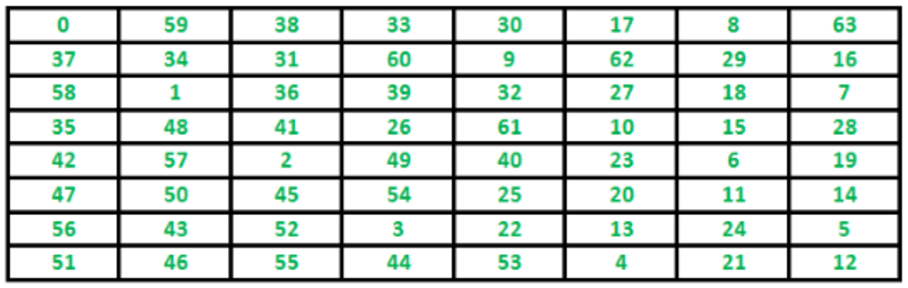
\includegraphics[width=0.8\textwidth]{Images/figGFGBkTSet1KnightsTour}
%\caption[]{}
%\label{figCXNX}
\end{figure}

Let us first discuss the na\"ive algorithm for this problem and then the
Backtracking algorithm.

\rrheader{Naive Algorithm for Knight's tour}

The na\"ive algorithm is to generate all tours one by one and check if the
generated tour satisfies the constraints.
\begin{lstlisting}[style=pseudostyle,numbers=none]
while there are untried tours
{ 
  generate the next tour 
  if this tour covers all squares 
  { 
    print this path;
  }
}
\end{lstlisting}
\textbf{Backtracking} works in an incremental way to attack problems.
Typically, we start from an empty solution vector and one by one add items
(the meaning of item varies from problem to problem. In context of Knight's
tour problem, \textbf{an item} is a \textbf{Knight's move}). When we add an
item, we check if adding the current item violates the problem constraint,
if it does then we remove the item and try other alternatives. \textbf{If
  none of the alternatives work out then we go to previous stage and remove
  the item added in the previous stage.} If we reach the initial stage back
then we say that no solution exists. If adding an item doesn't violate
constraints then we recursively add items one by one. If the solution vector
becomes complete then we print the solution.

\rrheader{Backtracking Algorithm for Knight's tour}

Following is the Backtracking algorithm for Knight's tour problem.
\begin{lstlisting}[style=pseudostyle,numbers=none]
If all squares are visited 
  print the solution
Else
  a) Add one of the next moves to solution vector and recursively 
  check if this move leads to a solution. (A Knight can make maximum 
  eight moves. We choose one of the 8 moves in this step).
  b) If the move chosen in the above step doesn't lead to a solution
  then remove this move from the solution vector and try other 
  alternative moves.
  c) If none of the alternatives work then return false (Returning false 
  will remove the previously added item in recursion and if false is 
  returned by the initial call of recursion then "no solution exists" )
\end{lstlisting}
Following are implementations for Knight's tour problem. It prints one of
the possible solutions in 2D matrix form. Basically, the output is a 2D
$8\times 8$ matrix with numbers from $0$ to $63$ and these numbers show
steps made by Knight.
\begin{lstlisting}[style=raycppnewsnippet]
// C program for Knight Tour problem
#include<stdio.h>
#define N 8
 
int solveKTUtil(int x, int y, int movei, int sol[N][N],
                int xMove[],  int yMove[]);
 
/* A utility function to check if i,j are valid indexes
   for N*N chessboard */
bool isSafe(int x, int y, int sol[N][N])
{
  return (x >= 0 && x < N && y >= 0 &&
          y < N && sol[x][y] == -1);
}
 
/* A utility function to print solution matrix sol[N][N] */
void printSolution(int sol[N][N])
{
  for (int x = 0; x < N; x++)
  {
    for (int y = 0; y < N; y++)
         printf(" %2d ", sol[x][y]);
    printf("\n");
  }
}

/* This function solves the Knight Tour problem using
   Backtracking.  This function mainly uses solveKTUtil()
   to solve the problem. It returns false if no complete
   tour is possible, otherwise return true and prints the
   tour.
   Please note that there may be more than one solutions,
   this function prints one of the feasible solutions.  */
bool solveKT()
{
  int sol[N][N];
 
  /* Initialization of solution matrix */
  for (int x = 0; x < N; x++)
      for (int y = 0; y < N; y++)
          sol[x][y] = -1;
 
  /* xMove[] and yMove[] define next move of Knight.
     xMove[] is for next value of x coordinate
     yMove[] is for next value of y coordinate */
  int xMove[8] = {  2, 1, -1, -2, -2, -1,  1,  2 };
  int yMove[8] = {  1, 2,  2,  1, -1, -2, -2, -1 };
 
  // Since the Knight is initially at the first block
  sol[0][0]  = 0;
 
  /* Start from 0,0 and explore all tours using
     solveKTUtil() */
  if (solveKTUtil(0, 0, 1, sol, xMove, yMove) == false)
  {
    printf("Solution does not exist");
    return false;
  }
  else
    printSolution(sol);
 
  return true;
}

/* A recursive utility function to solve Knight Tour
   problem */
int solveKTUtil(int x, int y, int movei, int sol[N][N],
                int xMove[N], int yMove[N])
{
  int k, next_x, next_y;
  if (movei == N*N)
    return true;
 
  /* Try all next moves from the current coordinate x, y */
  for (k = 0; k < 8; k++)
  {
    next_x = x + xMove[k];
    next_y = y + yMove[k];
    if (isSafe(next_x, next_y, sol))
    {
      sol[next_x][next_y] = movei;
      if (solveKTUtil(next_x, next_y, movei+1, sol,
                      xMove, yMove) == true)
        return true;
      else
        sol[next_x][next_y] = -1;// backtracking
    }
  }
  return false;
}
 
/* Driver program to test above functions */
int main()
{
  solveKT();
  return 0;
}
\end{lstlisting}
Output
\begin{lstlisting}[style=rayio]
  0  59  38  33  30  17   8  63
 37  34  31  60   9  62  29  16
 58   1  36  39  32  27  18   7
 35  48  41  26  61  10  15  28
 42  57   2  49  40  23   6  19
 47  50  45  54  25  20  11  14
 56  43  52   3  22  13  24   5
 51  46  55  44  53   4  21  12
\end{lstlisting}
Note that Backtracking is not the best solution for the Knight's tour
problem. See below article for other better solutions. The purpose of this
post is to explain Backtracking with an example.

Warnsdorff's algorithm for Knight's tour problem (see below).

References:
\begin{itemize}[noitemsep,topsep=0pt]
\item
  http://see.stanford.edu/materials/icspacs106b/H19-RecBacktrackExamples.pdf
\item
  http://www.cis.upenn.edu/~matuszek/cit594-2009/Lectures/35-backtracking.ppt
\item http://mathworld.wolfram.com/KnightsTour.html
\item http://en.wikipedia.org/wiki/Knight\%27s\_tour
\end{itemize}

\textbf{\rrgreen{Recommended: Please try your approach first, before moving
    on to the solution.}}

\RayNotesBegin

Here is my attempt, code here: \path{LeetCode/src/Bcktrck/rrrGFGBcktrckSet1KnightsTour.cpp}
\begin{lstlisting}[style=raycppnewsnippet]
// A utility function to check if (i,j) are valid indices
// for N*N chessboard
bool isLegal(const int x, const int y, const vector<vector<int>>& sol)
{
  auto N = static_cast<int>(sol.size());

  return ((x>=0) && (x<N) && (y>=0) && (y<N) &&
          (sol[x][y] == -1));
}

// A utility function to print a 2D vector
template<typename T>
void print2dVec(const vector<vector<T>>& vec, const string& str="")
{
  if(!str.empty())
  {
    cout << str;
  }

  for(const auto& row:vec)
  {
    for(const auto& val:row)
    {
      cout << std::setw(2) << val << ' ';
    }
    cout << '\n';
  }
}

// A recursive utility function to solve Knight Tour problem.
// curr_x and curr_y are the current x and y positions of the knight
// movei is a count of the current move number.
// sol contains the board.
// xMove and yMove are the new positions of the knight relative to current 
//   pos.
bool solveKTRecur(const int curr_x, const int curr_y, const int movei,
                  vector<vector<int>>& sol,
                  const vector<int>&xMove, const vector<int>&yMove)
{
  //cout << "Doing movei = " << movei << '\n';

  // Base case is when we have filled the whole board.
  // i.e. when movei == N*N
  auto N = static_cast<int>(sol.size());

  // The range of movei = [0..(N*N-1)]. However, for movei=N*N-1, we still
  // want to do the work (filling in the sol, if possible), so we test if
  // movei=N*N and return.
  if(movei == N*N) 
    return true;

  // Now loop through all the possibilities
  for(decltype(xMove.size()) i = 0; i < xMove.size(); ++i)
  {
    // create the next move
    int next_x = curr_x+xMove[i];
    int next_y = curr_y+yMove[i];

    // Check if this position is legal
    if(isLegal(next_x,next_y,sol))
    {
      // We know that we can place the next move here
      sol[next_x][next_y]=movei;

      // Now try every item from here.
      if(solveKTRecur(next_x,next_y,movei+1,
                      sol,xMove,yMove))
      {
        // we get here if we return true all the way down
        return true; 
      }
      else
      {
        // none of the 8 paths from here returns true. So we `backtrack'
        // this move/item and try the next of the 8 moves
        sol[next_x][next_y] = -1;
      }
    } // if legal
  } // for all items/moves

  // If we get here, it means that none of the items/moves worked. So we
  // return false.
  return false;
}

void runSolveKTRecur()
{
  // board size
  int N{8};
  
  // create the board and initialize with -1
  vector<vector<int>> board(N,vector<int>(N,-1));

  // start with the top left.
  int startx=0, starty=0;
  board[startx][starty]=0;

  // Create the eight moves in this order:
  //  2   1
  // 3     0
  //    x
  // 4     7
  //  5   6
  
  /* xMove[] and yMove[] define next move of Knight.
     xMove[] is for next value of x coordinate
     yMove[] is for next value of y coordinate */
  vector<int> xMove{2, 1, -1, -2, -2, -1,  1,  2};
  vector<int> yMove{1, 2,  2,  1, -1, -2, -2, -1};

  // If the solve returns true, it means there's a solution. Otherwise
  // there is no solution.
  if(solveKTRecur(startx,starty,1,board,xMove,yMove))
  {
    print2dVec(board, "Solution is:\n");
  }
  else
  {
    print2dVec(board, "No solution:\n");
    //cout << "Solution does not exist" << '\n';
  }

}

int main()
{
  runSolveKTRecur();

  return 0;
}
\end{lstlisting}

\RayNotesEnd

\textbf{\rrgreen{Back to geeksforgeeks solution.}}

Done, see above.



\subsection{Warnsdorff's algorithm for Knight's tour problem
  \label{secGFGBktrckKnightsTourWarnsdorff}}


RRRTODO

\url{http://www.geeksforgeeks.org/warnsdorffs-algorithm-knights-tour-problem/}

\textbf{Difficulty: 4.7}

\textbf{\rrgreen{Recommended: Please try your approach first, before moving
    on to the solution.}}

\RayNotesBegin



\RayNotesEnd

\textbf{\rrgreen{Back to geeksforgeeks solution.}}


%%%%%%%%%%%%%%%%%%%%%%%%%%%%%%%%%%%%%%%%%%%%%%%%%%%%%%%%%%%%%%%%%%%%%%%%%%%%
%%%%%%%%%%%%%%%%%%%%%%%%%%%%%%%%%%%%%%%%%%%%%%%%%%%%%%%%%%%%%%%%%%%%%%%%%%%%
%%%%%%%%%%%%%%%%%%%%%%%%%%%%%%%%%%%%%%%%%%%%%%%%%%%%%%%%%%%%%%%%%%%%%%%%%%%%

\section{Backtracking | Set 2 (Rat in a Maze)
  \label{secGFGBktrckSet2RatInMaze}}

\url{http://www.geeksforgeeks.org/backttracking-set-2-rat-in-a-maze}

\textbf{Difficulty: 3.2}

We have discussed Backtracking and Knight's tour problem in Set 1
(\pagecref{secGFGBktrckSet1KnightsTour}). Let us discuss Rat in a Maze as
another example problem that can be solved using Backtracking.

A Maze is given as N*N binary matrix of blocks where source block is the
upper left most block i.e., \ctt{maze[0][0]} and destination block is lower
rightmost block i.e., \ctt{maze[N-1][N-1]}. A rat starts from source and has
to reach destination. The rat can move only in two directions: forward and
down.

In the maze matrix, $0$ means the block is dead end and $1$ means the block
can be used in the path from source to destination. Note that this is a
simple version of the typical Maze problem. For example, a more complex
version can be that the rat can move in 4 directions and a more complex
version can be with limited number of moves.

Following is an example maze.

Gray blocks are dead ends (value = $0$). 

\begin{figure}
\centering
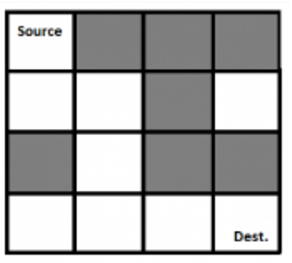
\includegraphics[width=0.3\textwidth]{Images/figGFGBkTSet2RatMaze1}
%\caption[]{}
%\label{figCXNX}
\end{figure}

Following is binary matrix representation of the above maze.
\begin{lstlisting}[style=raygeneric]
                {1, 0, 0, 0}
                {1, 1, 0, 1}
                {0, 1, 0, 0}
                {1, 1, 1, 1}
\end{lstlisting}
Following is maze with highlighted solution path.

\begin{figure}
\centering
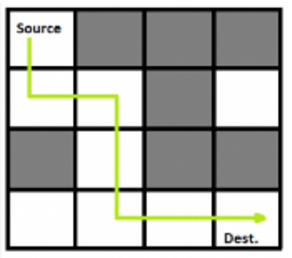
\includegraphics[width=0.3\textwidth]{Images/figGFGBkTSet2RatMaze2}
%\caption[]{}
%\label{figCXNX}
\end{figure}

Following is the solution matrix (output of program) for the above input
matrix.
\begin{lstlisting}[style=raygeneric]
                {1, 0, 0, 0}
                {1, 1, 0, 0}
                {0, 1, 0, 0}
                {0, 1, 1, 1}
\end{lstlisting}
All entries in solution path are marked as $1$.

\textbf{\rrgreen{Recommended: Please try your approach first, before moving
    on to the solution.}}

\RayNotesBegin

So the base case is when $(i,j)==(N-1,N-1)$. If we get to here, we return
\texttt{true}. The items are:
\begin{enumerate}[label=\textbf{\arabic*.}]
\item Go left: $(i,j)=(i+1,j)$.
\item Go down: $(i,j)=(i,j+1)$.
\end{enumerate}
Pseudocode:
\begin{lstlisting}[style=raygeneric]
When we loop through the items, we have to first check if it's legal.
Legal implies: the item is not a wall (value != 0) and is it within the
range of the maze.

  First we set the output value of this item to 1, and:
    Note that only the base case returns true, so we first check if the base
    case can be reached (therefore a solution is found) by recursively
    calling the algo, and propagate that true value back.

    Otherwise, we backtrack this item (set the value of the output to 0) and
    try the next item.

Out of the loop of items: If no true value is returned by any of the items,
we return false.
\end{lstlisting}
Let's code this up: \path{src/Bcktrck/rrrGFGBcktrckSet2RatInMaze.cpp}
\begin{lstlisting}[style=raycppnewsnippet]
template<typename T>
using Grid2d = vector<vector<T>>;

template<typename T>
void printGrid2d(const Grid2d<T>& grid, const string& str = "",
                 const int prec = 0)
{
  if(!str.empty())
    cout << str;

  for(const auto& row:grid)
  {
    for(const auto& val:row)
      cout << std::setw(prec) << val << ' ';
    cout << '\n';
  }
}

bool isLegal(const int x, const int y, const Grid2d<int>& maze)
{
  // size of the maze
  auto N = static_cast<int>(maze.size());

  return ((x >= 0)&&(x<N)&&(y>=0)&&(y<N)&&(maze[x][y] != 0));
}

bool solveMazeRecur(const int curr_x, const int curr_y,
                    const Grid2d<int>& maze,
                    const vector<int>& xmoves, const vector<int>& ymoves,
                    Grid2d<int>& sol)
{
  // size of the maze
  auto N = static_cast<int>(maze.size());

  // base case - solution found!
  if((curr_x == (N-1)) && (curr_y==(N-1)))
    return true;

  // Loop through the items and try each one.
  for(decltype(xmoves.size()) k = 0; k < xmoves.size(); ++k)
  {
    // Get the next position
    int next_x = curr_x + xmoves[k];
    int next_y = curr_y + ymoves[k];

    if(isLegal(next_x,next_y,maze))
    {
      // travel into the next path and ...
      sol[next_x][next_y] = 1;

      // ... try all paths from there
      if(solveMazeRecur(next_x,next_y,maze,xmoves,ymoves,sol))
      {
        return true;
      }
      else
      {
        // un-travel this item `backtracking' and try the next item
        sol[next_x][next_y] = 0;
      }
    }
  }

  // If none of the above child items returns true, then return false, 
  // indicating that this path should not be taken.
  return false;
}

void runSolveMazeRecur()
{
  Grid2d<int>maze{{1, 0, 0, 0},
                  {1, 1, 0, 1},
                  {0, 1, 0, 0},
                  {1, 1, 1, 1}};

  // Solution grid, initialized to 0
  auto N = maze.size();
  Grid2d<int>sol(N,vector<int>(N,0));

  // move vectors (the items), only right and down.
  vector<int> xmoves{1,0};
  vector<int> ymoves{0,1};

  // starting positions: top left.
  int start_x = 0, start_y = 0;
  sol[start_x][start_y] = 1;

  if(solveMazeRecur(start_x,start_y,maze,xmoves,ymoves,sol))
  {
    printGrid2d(sol,"Solution is:\n");
  }
  else
  {
    cout << "No solution.\n";
  }
}
int main()
{
  runSolveMazeRecur();
  return 0;
}
\end{lstlisting}

\RayNotesEnd

\textbf{\rrgreen{Back to geeksforgeeks solution.}}

\rrheader{Na\"ive Algorithm}

The Na\"ive Algorithm is to generate all paths from source to destination
and one by one check if the generated path satisfies the constraints.
\begin{lstlisting}[style=pseudostyle,numbers=none]
while there are untried paths
{
  generate the next path
  if this path has all blocks as 1
  {
    print this path;
  }
}
\end{lstlisting}

\rrheader{Backtrackng Algorithm}

\begin{lstlisting}[style=pseudostyle,numbers=none]
If destination is reached
  print the solution matrix
Else
  a) Mark current cell in solution matrix as 1. 
  b) Move forward in horizontal direction and recursively check if this 
      move leads to a solution. 
  c) If the move chosen in the above step doesn't lead to a solution
      then move down and check if  this move leads to a solution. 
  d) If none of the above solutions work then unmark this cell as 0 
      (BACKTRACK) and return false.
\end{lstlisting}
Implementation of Backtracking solution
\begin{lstlisting}[style=raycppnewsnippet]
/* C/C++ program to solve Rat in a Maze problem using
   backtracking */
#include<stdio.h>
 
// Maze size
#define N 4 
 
bool solveMazeUtil(int maze[N][N], int x, int y, int sol[N][N]);
 
/* A utility function to print solution matrix sol[N][N] */
void printSolution(int sol[N][N])
{
  for (int i = 0; i < N; i++)
  {
    for (int j = 0; j < N; j++)
      printf(" %d ", sol[i][j]);
    printf("\n");
  }
}
 
/* A utility function to check if x,y is valid index for N*N maze */
bool isSafe(int maze[N][N], int x, int y)
{
  // if (x,y outside maze) return false
  if(x >= 0 && x < N && y >= 0 && y < N && maze[x][y] == 1)
    return true;
 
  return false;
}

/* This function solves the Maze problem using Backtracking.  It mainly
   uses solveMazeUtil() to solve the problem. It returns false if no 
   path is possible, otherwise return true and prints the path in the
   form of 1s. Please note that there may be more than one solutions, 
   this function prints one of the feasible solutions.*/
bool solveMaze(int maze[N][N])
{
  int sol[N][N] = { {0, 0, 0, 0},
      {0, 0, 0, 0},
      {0, 0, 0, 0},
      {0, 0, 0, 0}
  };
 
  if(solveMazeUtil(maze, 0, 0, sol) == false)
  {
    printf("Solution doesn't exist");
    return false;
  }
 
  printSolution(sol);
  return true;
}

/* A recursive utility function to solve Maze problem */
bool solveMazeUtil(int maze[N][N], int x, int y, int sol[N][N])
{
  // if (x,y is goal) return true
  if(x == N-1 && y == N-1)
  {
    sol[x][y] = 1;
    return true;
  }
 
  // Check if maze[x][y] is valid
  if(isSafe(maze, x, y) == true)
  {
    // mark x,y as part of solution path
    sol[x][y] = 1;
 
    /* Move forward in x direction */
    if (solveMazeUtil(maze, x+1, y, sol) == true)
      return true;
 
    /* If moving in x direction doesn't give solution then
       Move down in y direction  */
    if (solveMazeUtil(maze, x, y+1, sol) == true)
      return true;
 
    /* If none of the above movements work then BACKTRACK: 
        unmark x,y as part of solution path */
    sol[x][y] = 0;
    return false;
  }   
 
  return false;
}

// driver program to test above function
int main()
{
  int maze[N][N]  =  { {1, 0, 0, 0},
                       {1, 1, 0, 1},
                       {0, 1, 0, 0},
                       {1, 1, 1, 1}};
 
  solveMaze(maze);
  return 0;
}
\end{lstlisting}
Output: The 1 values show the path for rat
\begin{lstlisting}[style=rayio]
 1  0  0  0 
 1  1  0  0 
 0  1  0  0 
 0  1  1  1 
\end{lstlisting}
Below is an extended version of this problem. Count number of ways to reach
destination in a Maze

%%%%%%%%%%%%%%%%%%%%%%%%%%%%%%%%%%%%%%%%%%%%%%%%%%%%%%%%%%%%%%%%%%%%%%%%%%%%
%%%%%%%%%%%%%%%%%%%%%%%%%%%%%%%%%%%%%%%%%%%%%%%%%%%%%%%%%%%%%%%%%%%%%%%%%%%%
%%%%%%%%%%%%%%%%%%%%%%%%%%%%%%%%%%%%%%%%%%%%%%%%%%%%%%%%%%%%%%%%%%%%%%%%%%%%

\subsection{Count number of ways to reach destination in a Maze
  \label{secGFGBktrckCountWaysMaze}}

\url{https://www.geeksforgeeks.org/count-number-ways-reach-destination-maze}

\textbf{Difficulty: 3.1}

RRRTODO


\textbf{\rrgreen{Recommended: Please try your approach first, before moving
    on to the solution.}}

\RayNotesBegin



\RayNotesEnd

\textbf{\rrgreen{Back to geeksforgeeks solution.}}


%%%%%%%%%%%%%%%%%%%%%%%%%%%%%%%%%%%%%%%%%%%%%%%%%%%%%%%%%%%%%%%%%%%%%%%%%%%%
%%%%%%%%%%%%%%%%%%%%%%%%%%%%%%%%%%%%%%%%%%%%%%%%%%%%%%%%%%%%%%%%%%%%%%%%%%%%
%%%%%%%%%%%%%%%%%%%%%%%%%%%%%%%%%%%%%%%%%%%%%%%%%%%%%%%%%%%%%%%%%%%%%%%%%%%%

\section{Backtracking | Set 3 (N Queen Problem)
  \label{secGFGBktrckSet3NQueenProb}}

\url{http://www.geeksforgeeks.org/backtracking-set-3-n-queen-problem}

\textbf{Difficulty: 3.5}

We have discussed Knight's tour and Rat in a Maze problems in Set 1
(\pagecref{secGFGBktrckSet1KnightsTour}) and Set 2
(\pagecref{secGFGBktrckSet2RatInMaze}) respectively. Let us discuss N Queen
as another example problem that can be solved using Backtracking.

The N Queen is the problem of placing $N$ chess queens on an $N\times N$
chessboard so that no two queens attack each other. For example, following
is a solution for $4$ Queen problem.

\begin{figure}
\centering
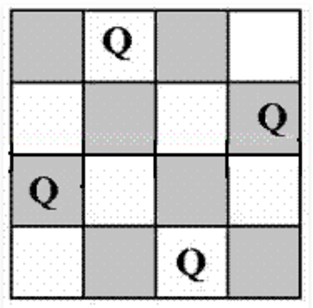
\includegraphics[width=0.25\textwidth]{Images/figGFGBkTSet3NQueen}
%\caption[]{}
%\label{figCXNX}
\end{figure}

The expected output is a binary matrix which has $1$s for the blocks where
queens are placed. For example following is the output matrix for above $4$
queen solution.
\begin{lstlisting}[style=raygeneric]
              { 0,  1,  0,  0}
              { 0,  0,  0,  1}
              { 1,  0,  0,  0}
              { 0,  0,  1,  0}
\end{lstlisting}

\textbf{\rrgreen{Recommended: Please try your approach first, before moving
    on to the solution.}}

\RayNotesBegin

Okay, let's recall what we know about backtracking.
\begin{itemize}[noitemsep,topsep=0pt]
\item We need to come up with the items/actions to take per recursive level.
\item We need to come up with the base case.
\item We need to come up with the restriction, which may depends on the
  previously places solution. This is usually handled by the \ctt{isLegal}
  method.
\end{itemize}

\textbf{Base case:} Easy, it's when we have placed $N$ queens on the board.

For the items, we need to use some logic. Let's place the first queen on the
top left, at $(i=0,j=0)$. Note that this is not fixed, so for the next
items, we can choose to place the queen (the initial one) at each of the
empty squares in row major order, and check if it's \emph{valid}. However,
we can do better. We know that since there are $N$ queens, and the board is
$N\times N$, then \textbf{each queen must be on its own column}.

Thus, we can work through the columns, for each column, the items are the
number of rows. We must check all rows, since the previously placed queens
may have moved (backtracked) to a different row. Say we work through the
columns from left to right, then to check if a square is valid, we only need
to check squares to the left:
\begin{itemize}[noitemsep,topsep=0pt]
\item Check squares to the left and see if there are no queens.
\item Check diagonal going up.
\item Check diagonal going down.
\end{itemize}
Thus, the pseudocode is something like this:
\begin{lstlisting}[style=pseudostyle,numbers=none]
bool solveNQueen(int col, grid sol[][])
{
  // We try to place the col-th queen. If col = sol.size(), then we know
  // that we have already placed all the N queens in the 0..N-1 columns.
  if(col == N)
    return true

  // Try to place the queen in the col-th column by looping throught the
  // rows
  Loop through rows
    if (row,col) is legal
      a) set the queen here: sol[row][col] = 1
      b) Go depth-first, recursively place the remaining queens, and
      propagate true back if a solution is reached.
      c) If it's not possible, then `backtrack' (reset) this row
         sol[row][col]=0
      and let the loop go for the next row.
    end if
  end loop through rows

  // If none of the rows work, return false.
  return false
}
\end{lstlisting}
Let's code this up: \path{Bcktrck/rrrGFGBcktrckSet3NQueen.cpp}
\begin{lstlisting}[style=raycppnewsnippet]
template<typename T>
using Grid2d = vector<vector<T>>;

template<typename T>
void printGrid2d(const Grid2d<T>& board)
{
  for(const auto& row:board)
  {
    for(const auto& val:row)
    {
      cout << val << ' ';
    }
    cout << '\n';
  }
}

// Check to see if x and y are within the board (0<=x,y<N-1) and 
// 1) Check left horizontally
// 2) Check up diagonal
// 3) Check down diagonal
bool isLegal(const int x, const int y, const Grid2d<int>& board)
{
  // First check if x and y are in range
  auto N = static_cast<int>(board.size());
  if(x < 0 || x>=N || y<0 || y>= N)
  {
    return false;
  }

  // Check if to the left, so only column changes
  for(int yi = 0; yi < y; ++yi)
    if(board[x][yi] == 1)
      return false;

  // Check if up diag, both row and col indices reduce by 1 at each 
  // iteration
  for(int xi = x, yi = y; xi >= 0 && yi >= 0; xi--, yi--)
    if(board[xi][yi]==1)
      return false;

  // Check if down diag, row increases by 1, col decreases by 1
  for(int xi = x, yi = y; xi < N && yi >= 0; ++xi, --yi)
    if(board[xi][yi]==1)
      return false;

  return true;
}

bool solveNQueenRecur(const int col, Grid2d<int>& board)
{
  // We try to place the col-th queen in the col-th column. 
  // If col == board.size(), then we know that we have already placed all 
  // the N queens in the 0..N-1 columns
  auto N = static_cast<int>(board.size());
  if(col == N)
    return true;

  // Try to place the queen in the col-th column by looping through the rows
  for(int row = 0; row < N; ++row)
  {
    if(isLegal(row,col,board))
    {
      // Found a legal square, so we set the queen here
      board[row][col] = 1;
      
      // Now try for the next column. We go deeper, depth-first,
      // recursively placing the remaining queens, and propagate true back
      // to the caller of this function if the base case is reached.
      if(solveNQueenRecur(col+1,board))
        return true;
      else
        // backtrack by resetting (row,col) to zero, so we can try a 
        // different row.
        board[row][col] = 0;
    }
  }

  // If none of the rows work=>none of the path of items , return false
  return false;
}

void runSolveNQueens()
{
  constexpr size_t N = 100;
  Grid2d<int> board(N,vector<int>(N,0));
  solveNQueenRecur(0,board);
  printGrid2d(board);
}

int main()
{
  runSolveNQueens();
  return 0;
}
\end{lstlisting}

\RayNotesEnd

\textbf{\rrgreen{Back to geeksforgeeks solution.}}

\rrheader{Naive Algorithm}

Generate all possible configurations of queens on board and print a
configuration that satisfies the given constraints.
\begin{lstlisting}[style=pseudostyle,numbers=none]
while there are untried conflagrations
{
  generate the next configuration
  if queens don't attack in this configuration then
  {
    print this configuration;
  }
}
\end{lstlisting}

\rrheader{Backtracking Algorithm}

The idea is to place queens one by one in different columns, starting from
the leftmost column. When we place a queen in a column, we check for clashes
with already placed queens. In the current column, if we find a row for
which there is no clash, we mark this row and column as part of the
solution. If we do not find such a row due to clashes then we backtrack and
return \texttt{false}.
\begin{lstlisting}[style=raygeneric]
1) Start in the leftmost column
2) If all queens are placed
    return true
3) Try all rows in the current column.  Do following for every tried row.
    a) If the queen can be placed safely in this row then mark this [row, 
        column] as part of the solution and recursively check if placing  
        queen here leads to a solution.
    b) If placing queen in [row, column] leads to a solution then return 
        true.
    c) If placing queen doesn't lead to a solution then umark this [row, 
        column] (Backtrack) and go to step (a) to try other rows.
3) If all rows have been tried and nothing worked, return false to trigger 
    backtracking.
\end{lstlisting}

\rrheader{Implementation of Backtracking solution}

\begin{lstlisting}[style=raycppnewsnippet]
/* C/C++ program to solve N Queen Problem using
   backtracking */
#define N 4
#include<stdio.h>
 
/* A utility function to print solution */
void printSolution(int board[N][N])
{
  for (int i = 0; i < N; i++)
  {
    for (int j = 0; j < N; j++)
      printf(" %d ", board[i][j]);
    printf("n");
  }
}

/* A utility function to check if a queen can
   be placed on board[row][col]. Note that this
   function is called when "col" queens are
   already placed in columns from 0 to col -1.
   So we need to check only left side for
   attacking queens */
bool isSafe(int board[N][N], int row, int col)
{
  int i, j;
 
  /* Check this row on left side */
  for (i = 0; i < col; i++)
    if (board[row][i])
      return false;
 
  /* Check upper diagonal on left side */
  for (i=row, j=col; i>=0 && j>=0; i--, j--)
    if (board[i][j])
      return false;
 
  /* Check lower diagonal on left side */
  for (i=row, j=col; j>=0 && i<N; i++, j--)
    if (board[i][j])
      return false;
 
  return true;
}

/* A recursive utility function to solve N
   Queen problem */
bool solveNQUtil(int board[N][N], int col)
{
  /* base case: If all queens are placed
    then return true */
  if (col >= N)
    return true;
 
  /* Consider this column and try placing
     this queen in all rows one by one */
  for (int i = 0; i < N; i++)
  {
    /* Check if queen can be placed on
      board[i][col] */
    if ( isSafe(board, i, col) )
    {
      /* Place this queen in board[i][col] */
      board[i][col] = 1;
 
      /* recur to place rest of the queens */
      if ( solveNQUtil(board, col + 1) )
        return true;
 
      /* If placing queen in board[i][col]
         doesn't lead to a solution, then
         remove queen from board[i][col] */
      board[i][col] = 0; // BACKTRACK
    }
  }
 
   /* If queen can not be place in any row in
      this colum col  then return false */
  return false;
}

/* This function solves the N Queen problem using
   Backtracking. It mainly uses solveNQUtil() to
   solve the problem. It returns false if queens
   cannot be placed, otherwise return true and
   prints placement of queens in the form of 1s.
   Please note that there may be more than one
   solutions, this function prints one  of the
   feasible solutions.*/
bool solveNQ()
{
  int board[N][N] = { {0, 0, 0, 0},
      {0, 0, 0, 0},
      {0, 0, 0, 0},
      {0, 0, 0, 0}
  };
 
  if ( solveNQUtil(board, 0) == false )
  {
    printf("Solution does not exist");
    return false;
  }
 
  printSolution(board);
  return true;
}
 
// driver program to test above function
int main()
{
  solveNQ();
  return 0;
}
\end{lstlisting}
Output: The 1 values indicate placements of queens
\begin{lstlisting}[style=rayio]
 0  0  1  0 
 1  0  0  0 
 0  0  0  1 
 0  1  0  0 
\end{lstlisting}

Sources:
\begin{itemize}[noitemsep,topsep=0pt]
\item
  http://see.stanford.edu/materials/icspacs106b/H19-RecBacktrackExamples.pdf
\item http://en.literateprograms.org/Eight\_queens\_puzzle\_\%28C\%29
\item http://en.wikipedia.org/wiki/Eight\_queens\_puzzle
\end{itemize}

%%%%%%%%%%%%%%%%%%%%%%%%%%%%%%%%%%%%%%%%%%%%%%%%%%%%%%%%%%%%%%%%%%%%%%%%%%%%
%%%%%%%%%%%%%%%%%%%%%%%%%%%%%%%%%%%%%%%%%%%%%%%%%%%%%%%%%%%%%%%%%%%%%%%%%%%%
%%%%%%%%%%%%%%%%%%%%%%%%%%%%%%%%%%%%%%%%%%%%%%%%%%%%%%%%%%%%%%%%%%%%%%%%%%%%

\subsection{Printing all solutions in N-Queens Problem}

\url{https://www.geeksforgeeks.org/printing-solutions-n-queen-problem}

\textbf{Difficulty: 3.6}

The N Queen is the problem of placing N chess queens on an $N\times N$
chessboard so that no two queens attack each other. For example, following
is a solution for 4 Queen problem.

The N Queen is the problem of placing N chess queens on an $N\times N$
chessboard so that no two queens attack each other. For example, following
is a solution for 4 Queen problem.

\begin{figure}
\centering
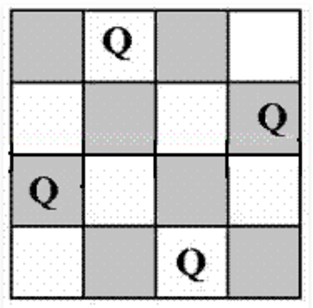
\includegraphics[width=0.25\textwidth]{Images/figGFGBkTSet3NQueen}
%\caption[]{}
%\label{figCXNX}
\end{figure}

In previous post, we have discussed an approach that prints only one
possible solution, so now in this post the task is to print all solutions in
N-Queen Problem. The solution discussed here is an extension of same
approach.

\textbf{\rrgreen{Recommended: Please try your approach first, before moving
    on to the solution.}}

\RayNotesBegin

RRRTODO - it seems pretty easy. It's literally looping through all the
rows rather than returning at the first sight of a solution. And we always
backtrack. This seems more like a brute force approach than anything else.

\RayNotesEnd

\textbf{\rrgreen{Back to geeksforgeeks solution.}}



%%%%%%%%%%%%%%%%%%%%%%%%%%%%%%%%%%%%%%%%%%%%%%%%%%%%%%%%%%%%%%%%%%%%%%%%%%%%
%%%%%%%%%%%%%%%%%%%%%%%%%%%%%%%%%%%%%%%%%%%%%%%%%%%%%%%%%%%%%%%%%%%%%%%%%%%%
%%%%%%%%%%%%%%%%%%%%%%%%%%%%%%%%%%%%%%%%%%%%%%%%%%%%%%%%%%%%%%%%%%%%%%%%%%%%

\section{Backtracking | Set 4 (Subset Sum)
  \label{secGFGBktrckSet4SubsetSum}}

\url{http://www.geeksforgeeks.org/backttracking-set-4-subset-sum}

\textbf{Difficulty: 4.4}

Subset sum problem is to find subset of elements that are selected from a
given set whose sum adds up to a given number $K$. We are considering the
set contains non-negative values. It is assumed that the input set is unique
(no duplicates are presented).

\textbf{\rrgreen{Recommended: Please try your approach first, before moving
    on to the solution.}}

\RayNotesBegin

I really don't this the backtracking solution to this atm. So I'll just go
onto the solution. However, note that this can be easily solved by DP, it's
basically an integer partitioning. We have a sum, and have to partition it
into some subset of integers, see this:\\
\url{https://www.geeksforgeeks.org/dynamic-programming-subset-sum-problem}

\RayNotesEnd

\textbf{\rrgreen{Back to geeksforgeeks solution.}}

\rrheader{Exhaustive Search Algorithm for Subset Sum}

One way to find subsets that sum to $K$ is to consider all possible subsets.
A power set contains all those subsets generated from a given set. The size
of such a power set is $2^N$.

\rrheader{Backtracking Algorithm for Subset Sum}

Using exhaustive search we consider all subsets irrespective of whether they
satisfy given constraints or not. Backtracking can be used to make a
systematic consideration of the elements to be selected.

\rrblue{(But how do we select them using backtracking? What are the "items"
  - how do we generate them?)}

Assume given set of $4$ elements, say $w[1]\ldots w[4]$. Tree diagrams can
be used to design backtracking algorithms. The following tree diagram
depicts approach of generating variable sized tuple.

\begin{figure}
\centering
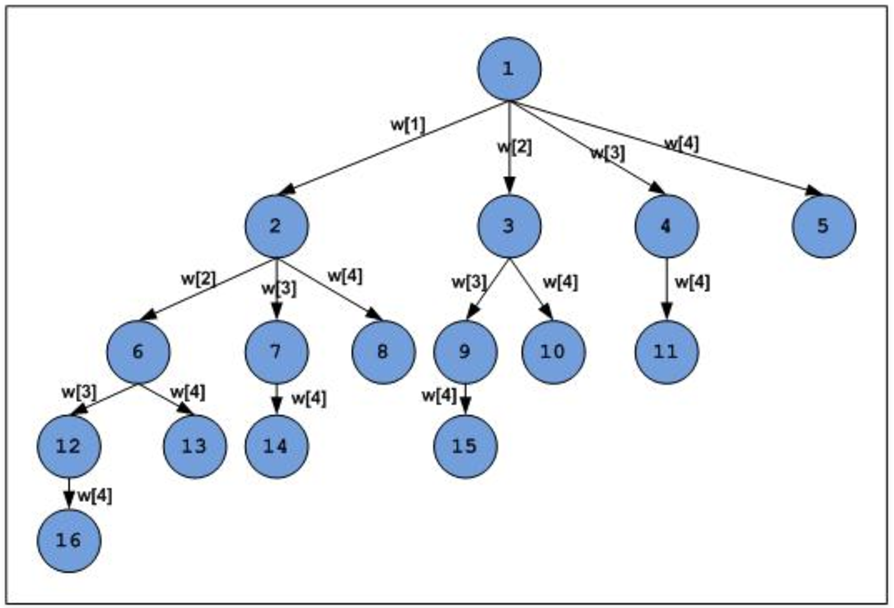
\includegraphics[width=0.8\textwidth]{Images/figGFGBkTSet4SubsetSum}
%\caption[]{}
%\label{figCXNX}
\end{figure}

In the above tree, a node represents function call and a branch represents
candidate element. The root node contains 4 children. In other words, the
root considers every element of the set as different branch. The next level
\textbf{sub-trees} correspond to the subsets that includes the parent node.
The branches at each level represent tuple elements to be considered. For
example, if we are at level 1, \ctt{tuple\_vector[1]} can take any value of
four branches generated. If we are at level 2 of left most node,
\ctt{tuple\_vector[2]} can take any value of three branches generated, and
so on...

For example the left most child of the root generates all those subsets that
include \ctt{w[1]}. Similarly the second child of root generates all those
subsets that includes \ctt{w[2]} \textbf{and excludes} \ctt{w[1]}.

As we go down along depth of tree we add elements so far, and if the added
sum is satisfying \textbf{explicit constraints}, we will continue to
generate child nodes further. Whenever the constraints are not met, we stop
further generation of sub-trees of that node, and backtrack to previous node
to explore the nodes not yet explored. In many scenarios, it saves
considerable amount of processing time.

The tree should trigger a clue to implement the backtracking algorithm (try
yourself). It prints all those subsets whose sum add up to given number. We
need to explore the nodes along the breadth and depth of the tree.
Generating nodes along breadth is controlled by loop and nodes along the
depth are generated using recursion (post order traversal). Pseudo code
given below,
\begin{lstlisting}[style=raygeneric]
if(subset is satisfying the constraint)
  print the subset
  exclude the current element and consider next element
else
  generate the nodes of present level along breadth of tree and
  recur for next levels
\end{lstlisting}
Following is C implementation of subset sum using variable size tuple
vector. Note that the following program explores all possibilities similar
to exhaustive search. It is to demonstrate how backtracking can be used. See
next code to verify, how we can optimize the backtracking solution.

For my attempt see here:\\
\path{src/Bcktrck/rrrGFGBcktrckSet4SubsetSum.cpp}\\
also see their solution at:\\
\path{src/Bcktrck/rrrGFGBcktrckSet4Test.cpp}\\

I'll come back to this, since I cba... it jut seems a bit weird.

RRRTODO

%%%%%%%%%%%%%%%%%%%%%%%%%%%%%%%%%%%%%%%%%%%%%%%%%%%%%%%%%%%%%%%%%%%%%%%%%%%%
%%%%%%%%%%%%%%%%%%%%%%%%%%%%%%%%%%%%%%%%%%%%%%%%%%%%%%%%%%%%%%%%%%%%%%%%%%%%
%%%%%%%%%%%%%%%%%%%%%%%%%%%%%%%%%%%%%%%%%%%%%%%%%%%%%%%%%%%%%%%%%%%%%%%%%%%%

\section{Backtracking | Set 5 (m Coloring Problem)
  \label{secGFGBktrckSet5mColorProb}}

\url{http://www.geeksforgeeks.org/backttracking-set-5-m-coloring-problem}

\textbf{Difficulty: 3.6}

Given an undirected graph and a number $m$, determine if the graph can be
colored with at most $m$ colors such that no two adjacent vertices of the
graph are colored with same color. Here coloring of a graph means assignment
of colors to all vertices.

\noindent{}\textbf{Input:}\\
\begin{enumerate}[label=\textbf{\arabic*.}]
\item A 2D array \ctt{graph[V][V]} where $V$ is the number of vertices in
  graph and \ctt{graph[V][V]} is adjacency matrix representation of the
  graph. A value \ctt{graph[i][j]} is $1$ if there is a direct edge from $i$
  to $j$, otherwise \ctt{graph[i][j]} is $0$.
\item An integer $m$ which is maximum number of colors that can be used.
\end{enumerate}

\noindent{}\textbf{Output:}\\
An array \ctt{color[V]} that should have numbers from $1$ to $m$.
\ctt{color[i]} should represent the color assigned to the $i$th vertex. The
code should also return false if the graph cannot be colored with $m$
colors.

Following is an example graph (from Wiki page ) that can be colored with 3
colors.

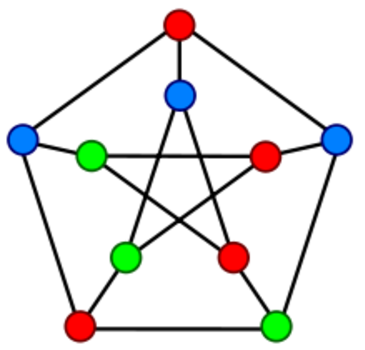
\includegraphics[width=0.3\textwidth]{Images/figGFGBkTSet5GraphColor}

\textbf{\rrgreen{Recommended: Please try your approach first, before moving
    on to the solution.}}

\RayNotesBegin

When you can't think of a solution or approach to a problem, it might help
to come up with the brute-force solution, and then maybe a simpler example,
a reduced problem.

\noindent{}\textbf{Brute force:} Try every combination of colouring, and
check which one satisfies the constraint. Since each node can be one of $m$
colours, so there are $m^N$ different combinations of colouring, where $N$
is the number of nodes in the graph (i.e. if there are only 2 colours, then
it's $2^N$, which is the same as the number of different combinations of
binary numbers of $N$ bits).

So trying each combination of colours is the ``item'', which spans the
breadth. We start at node $i=0$, and set it to a color $color[i]=c, c\in
[1..m]$, check if it's legal. Legal means that no other node in the
adjacency matrix has the same color as color $c$. If it's legal, then we
recursively try to update $color[i+1]$. If not, we backtrack, setting
\ctt{color[i]=0} and trying the next color in the loop.

Let's code this up:
\begin{lstlisting}[style=raycppnewsnippet]
template<typename T>
using Grid2d = vector<vector<T>>;

// function to output a vector
template<typename T>
void printVec(vector<T>& v, const string& str="")
{
  if(!str.empty()) cout << str;
  for(const auto& val:v)
    cout << val << " ";
  cout << '\n';
}

// a color m_index is legal for nodei is no other node in graph[nodei] has
// the same color
bool isLegal(const int nodei, const int m_index, 
             const Grid2d<int>& graph, const vector<int>& color)
{
  // Loop through the nodes, if they are adjacent to node i, check if
  // it has been assigned a color the same as color[m_index]
  for(size_t i = 0; i < graph.size(); ++i)
    if(graph[nodei][i] && (m_index==color[i]))
      return false;
  
  return true;
}

bool solveMColor(const Grid2d<int>& graph, const int m, const int nodei, 
                  vector<int>& color)
{
  // base case is when we have coloured all the nodes, i.e.
  // when nodei = color.size()
  if(nodei == color.size())
    return true;

  // For this node, loop through the colors, backtrack is necessary 
  // (breadth-first).
  // Recursively call solveMColor for node+1 (depth-first)
  for(int m_index = 1; m_index <= m; m_index++)
  {
    if(isLegal(nodei, m_index, graph, color))
    {
      color[nodei] = m_index;
      if(solveMColor(graph, m, nodei+1, color))
        return true;

      // backtrack
      color[nodei] = 0;
    }
  }

  return false;
}

void runSolveMColor()
{
  Grid2d<int> grid{{0,1,1,1},
                   {1,0,1,0},
                   {1,1,0,1},
                   {1,0,1,0}};

  int m = 3;
  vector<int> color(grid.size(),0);

  if(solveMColor(grid, m, 0, color))
    printVec(color,"Solution is:\n");
  else
    cout << "No sol" << '\n';
}

int main()
{
  runSolveMColor();
  return 0;
}
\end{lstlisting}

\RayNotesEnd

\textbf{\rrgreen{Back to geeksforgeeks solution.}}

\rrheader{Naive Algorithm}

Generate all possible configurations of colors and print a configuration
that satisfies the given constraints.
\begin{lstlisting}[style=raycppnewsnippet]
while there are untried conflagrations
{
  generate the next configuration
  if no adjacent vertices are colored with same color
  {
    print this configuration;
  }
}
\end{lstlisting}
There will be $m^V$ configurations of colors.

\rrheader{Backtracking Algorithm}

The idea is to assign colors one by one to different vertices, starting from
the vertex $0$. Before assigning a color, we check for safety by considering
already assigned colors to the adjacent vertices. If we find a color
assignment which is safe, we mark the color assignment as part of solution.
If we do not a find color due to clashes then we backtrack and return
\texttt{false}.

Implementation of Backtracking solution
\begin{lstlisting}[style=raycppnewsnippet]
#include<stdio.h>
 
// Number of vertices in the graph
#define V 4
 
void printSolution(int color[]);
 
/* A utility function to check if the current color assignment
   is safe for vertex v */
bool isSafe (int v, bool graph[V][V], int color[], int c)
{
  for (int i = 0; i < V; i++)
    if (graph[v][i] && c == color[i])
      return false;
  return true;
}
 
/* A recursive utility function to solve m coloring problem */
bool graphColoringUtil(bool graph[V][V], int m, int color[], int v)
{
  /* base case: If all vertices are assigned a color then
       return true */
  if (v == V)
    return true;
 
  /* Consider this vertex v and try different colors */
  for (int c = 1; c <= m; c++)
  {
    /* Check if assignment of color c to v is fine*/
    if (isSafe(v, graph, color, c))
    {
      color[v] = c;

      /* recur to assign colors to rest of the vertices */
      if (graphColoringUtil (graph, m, color, v+1) == true)
        return true;
 
      /* If assigning color c doesn't lead to a solution
         then remove it */
      color[v] = 0;
    }
  }
 
  /* If no color can be assigned to this vertex then return false */
  return false;
}
 
/* This function solves the m Coloring problem using Backtracking.
  It mainly uses graphColoringUtil() to solve the problem. It returns
  false if the m colors cannot be assigned, otherwise return true and
  prints assignments of colors to all vertices. Please note that there
  may be more than one solutions, this function prints one of the
  feasible solutions.*/
bool graphColoring(bool graph[V][V], int m)
{
  // Initialize all color values as 0. This initialization is needed
  // correct functioning of isSafe()
  int *color = new int[V];
  for (int i = 0; i < V; i++)
    color[i] = 0;
 
  // Call graphColoringUtil() for vertex 0
  if (graphColoringUtil(graph, m, color, 0) == false)
  {
    printf("Solution does not exist");
    return false;
  }
 
  // Print the solution
  printSolution(color);
  return true;
}
 
/* A utility function to print solution */
void printSolution(int color[])
{
  printf("Solution Exists:"
         " Following are the assigned colors \n");
  for (int i = 0; i < V; i++)
    printf(" %d ", color[i]);
  printf("\n");
}
 
// driver program to test above function
int main()
{
  /* Create following graph and test whether it is 3 colorable
    (3)---(2)
     |   / |
     |  /  |
     | /   |
    (0)---(1)
  */
  bool graph[V][V] = {{0, 1, 1, 1},
                      {1, 0, 1, 0},
                      {1, 1, 0, 1},
                      {1, 0, 1, 0},
                     };
  int m = 3; // Number of colors
  graphColoring (graph, m);
  return 0;
}
\end{lstlisting}
Output:
\begin{lstlisting}[style=rayio]
Solution Exists: Following are the assigned colors
 1  2  3  2
\end{lstlisting}
References:
\url{http://en.wikipedia.org/wiki/Graph\_coloring}

%%%%%%%%%%%%%%%%%%%%%%%%%%%%%%%%%%%%%%%%%%%%%%%%%%%%%%%%%%%%%%%%%%%%%%%%%%%%
%%%%%%%%%%%%%%%%%%%%%%%%%%%%%%%%%%%%%%%%%%%%%%%%%%%%%%%%%%%%%%%%%%%%%%%%%%%%
%%%%%%%%%%%%%%%%%%%%%%%%%%%%%%%%%%%%%%%%%%%%%%%%%%%%%%%%%%%%%%%%%%%%%%%%%%%%

\section{Backtracking | Set 6 (Hamiltonian Cycle)
  \label{secGFGBktrckSet6HamiltonianCycle}}

\url{http://www.geeksforgeeks.org/backtracking-set-7-hamiltonian-cycle}

\textbf{Difficulty: 3.7}

\textbf{\emph{Hamiltonian
    Path}}\footnote{\url{http://en.wikipedia.org/wiki/Hamiltonian\_path}}
in an undirected graph is a path that \textbf{visits each vertex exactly
  once}. A \textbf{\emph{Hamiltonian cycle}} (or Hamiltonian circuit) is a
Hamiltonian Path such that there is an edge (in the graph) from the last
vertex to the first vertex of the Hamiltonian Path. Determine whether a
given graph contains Hamiltonian Cycle or not. If it contains, then print
the path. Following are the input and output of the required function.

\noindent{}\textbf{Input:}\\
A 2D array \ctt{graph[V][V]} where $V$ is the number of vertices in the
graph and \ctt{graph[V][V]} is adjacency matrix representation of the graph.
A value \ctt{graph[i][j]} is $1$ if there is a direct edge from $i$ to $j$,
otherwise \ctt{graph[i][j]} is $0$.

\noindent{}\textbf{Output:}\\ An array \ctt{path[V]} that should contain the
Hamiltonian Path.  \ctt{path[i]} should represent the $i$th vertex in the
Hamiltonian Path. The code should also return \texttt{false} if there is no
Hamiltonian Cycle in the graph.

For example, a Hamiltonian Cycle in the following graph is
$\set*{0,1,2,4,3,0}$. There are more Hamiltonian Cycles in the graph like
$\set*{0,3,4,2,1,0}$
\begin{lstlisting}[style=raygeneric]
(0)--(1)--(2)
 |   / \   |
 |  /   \  | 
 | /     \ |
(3)-------(4)
\end{lstlisting}
And the following graph doesn't contain any Hamiltonian Cycle.
\begin{lstlisting}[style=raygeneric]
(0)--(1)--(2)
 |   / \   |
 |  /   \  | 
 | /     \ |
(3)      (4) 
\end{lstlisting}

\textbf{\rrgreen{Recommended: Please try your approach first, before moving
    on to the solution.}}

\RayNotesBegin

This is a bit more complicated than the last one since there is an
additional condition on the last node (it has to be adjacent to the first
node).

First, let's jot some notes down, then describe the naive approach.
\begin{itemize}[noitemsep,topsep=0pt]
\item The choices of nodes are the items in this case.
\item We start with node $0$, this is justified since we're forming a cycle,
  so it does not matter where we start. This is what we start the recursion
  with.
\item At each node (level of recursion) (this is the breadth-first stage),
  we loop through the node's adjacency list, generating the breadth-first
  items.
\item For each of the breadth-first items (adjacency nodes), we check if
  it's \textbf{legal}. In this case, legal means that we have not visited
  the node already. This is easily done since we have a list of nodes we
  have visited in the array \ctt{path[V]}, thus we simply which if the node
  we're going to add to the \ctt{path} is not already in \ctt{path}.
\item For the \textbf{base case}, we do not simply check if we have
  \textbf{already} added all the nodes to \ctt{path}. (For which we check if
  the node we're trying to add is equal to the number of nodes). Instead, we
  check if check if this is the last node to be added (nodei==V-1), if so,
  we check if the first node is in the adjacency list of nodei. If it is,
  then we're done, return \texttt{true}. If not, then a cycle cannot be
  formed on this path, so we return \texttt{false}.
\end{itemize}

Let's code this up!
Done, but with a small bug with I cba to find. The code is here:\\
\path{src/Bcktrck/rrrGFGBcktrckSet6Hamiltonian.cpp}

\RayNotesEnd

\textbf{\rrgreen{Back to geeksforgeeks solution.}}





%%%%%%%%%%%%%%%%%%%%%%%%%%%%%%%%%%%%%%%%%%%%%%%%%%%%%%%%%%%%%%%%%%%%%%%%%%%%
%%%%%%%%%%%%%%%%%%%%%%%%%%%%%%%%%%%%%%%%%%%%%%%%%%%%%%%%%%%%%%%%%%%%%%%%%%%%
%%%%%%%%%%%%%%%%%%%%%%%%%%%%%%%%%%%%%%%%%%%%%%%%%%%%%%%%%%%%%%%%%%%%%%%%%%%%

\section{Backtracking | Set 7 Sudoku
  \label{secGFGBktrckSet7Sudoku}}

\url{http://www.geeksforgeeks.org/backtracking-set-7-suduku}

\textbf{Difficulty: 3.8}

Given a partially filled $9\times 9$ 2D array `\ctt{grid[9][9]}', the goal
is to assign digits (from $1$ to $9$) to the empty cells so that every row,
column, and subgrid of size $3\times 3$ contains exactly one instance of the
digits from $1$ to $9$.

\begin{figure}
\centering
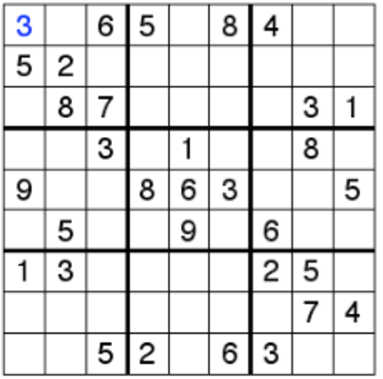
\includegraphics[width=0.3\textwidth]{Images/figGFGBkTSet7Sudoku}
%\caption[]{}
%\label{figCXNX}
\end{figure}

\textbf{\rrgreen{Recommended: Please try your approach first, before moving
    on to the solution.}}

\RayNotesBegin

I'll do it alongside the solution to save time. This seems pretty easy. It's
standard backtracking.

\RayNotesEnd

\textbf{\rrgreen{Back to geeksforgeeks solution.}}

\rrheader{Naive Algorithm}

The Naive Algorithm is to generate all possible configurations of numbers
from 1 to 9 to fill the empty cells. Try every configuration one by one
until the correct configuration is found.

\rrheader{Backtracking Algorithm}

Like all other Backtracking problems, we can solve Sudoku by one by one
assigning numbers to empty cells. Before assigning a number, we check
whether it is safe to assign. We basically check that the same number is not
present in \textbf{current row}, \textbf{current column} and current
$3\times 3$ subgrid. After checking for safety, we assign the number, and
recursively check whether this assignment leads to a solution or not. If the
assignment doesn't lead to a solution, then we try next number for current
empty cell. And if none of number ($1$ to $9$) lead to solution, we return
\texttt{false}.

\begin{lstlisting}[style=raygeneric]
Find row, col of an unassigned cell
  If there is none, return true // base case!
  
  For digits from 1 to 9
    a) If there is no conflict for digit at row,col
        assign digit to row,col and recursively try fill in rest of grid
    b) If recursion successful, return true
    c) Else, remove digit and try another
  
  If all digits have been tried and nothing worked, return false
\end{lstlisting}

Following are C++ and Python implementation for Sudoku problem. It prints
the completely filled grid as output. This is my own version, located at
\path{src/Bcktrck/rrrGFGBcktrckSet7Sudoku.cpp}. See the GFG website for
theirs.
\begin{lstlisting}[style=raycppnewsnippet]
// UNASSIGNED is used for empty cells in sudoku grid
static constexpr int UNASSIGNED{0};

// N is used for the size of the sudoku grid. Size will be NxN
static constexpr int GridSize{9};

template<typename T>
using Grid2d = vector<vector<T>>;

// A utility function to print grid
template<typename T>
void printGrid(const Grid2d<T>& grid, string str="")
{
  if(!str.empty()) cout << str;
  for(const auto& row:grid)
  {
    for(const auto& val:row)
      cout << val << " ";
    cout << '\n';
  }
}

// Searches the grid to find an entry that is still unassigned. If found, 
// the reference parameters row, col will be set to the location that is
// unassigned, and true is returned. If no assigned entries remain, false
// is returned.
bool FindUnassignedLocation(const Grid2d<int>& grid, int& row, int& col)
{
  for(row = 0; row < GridSize; ++row)
    for(col = 0; col < GridSize; ++col)
      if(grid[row][col] == UNASSIGNED)
        return true;
  return false;
}

// Functions to check if it's legal (isSafe), to do this, we need to check
// if the number is (1) used in the row, (2) used in the column, and (3)
// used in the box

// Returns a boolean which indicates whether any assigned entry in the 
// specified row matches the given number
bool UsedInRow(const Grid2d<int>& grid, const int row, const int num)
{
  return std::find(grid[row].begin(),grid[row].end(),num) != grid[row].end();
}

// Returns a boolean which determines whether any assigned entry in the
// specified column matches the give number.
bool UsedInCol(const Grid2d<int>& grid, const int col, const int num)
{
  // Loop through the rows of a given col
  for(int row = 0; row < GridSize; ++row)
    if(grid[row][col]==num)
      return true;
  return false;
}

// Returns a boolean which indicates whether any assigned entry within the
// specified 3x3 box matches the given number.
bool UsedInBox(const Grid2d<int>& grid, const int boxStartRow, 
               const int boxStartCol, const int num)
{
  for(int row=0; row < 3; ++row)
    for(int col=0; col < 3; ++col)
      if(grid[boxStartRow+row][boxStartCol+col] == num)
        return true;
  return false;
}

// Returns a boolean which indicates whether it will be legal to assign num
// to the given (row,col) location
bool isSafe(const Grid2d<int>& grid, const int row, const int col, 
            const int num)
{
  // Check if 'num' is not already placed in the current row, current 
  // column, and current 3x3 box
  return !UsedInRow(grid, row, num) &&
         !UsedInCol(grid, col, num) &&
         !UsedInBox(grid, row-row%3, col-col%3, num);
  // The last part makes sense, since, e.g.
  // 0, 1, 2 | 3, 4, 5 | 6, 7, 8
  //
  // Take the middle square, if we have 3, then:
  // 5-5%3 = 5-2=3 | 3(+2)-2=3
  // 4-4%3 = 4-1=3 | 3(+1)-1=3
  // 3-3%3 = 3-0=3 | 3(+0)-0=3
}

// Takes a partially filled-in grid and attempts to assign values to all 
// unassigned locations in such a way to meet the requirements for Sudoku
// solution (non-duplication across rows, columns, and boxes)
bool solveSudoku(Grid2d<int>& grid)
{
  int row, col;

  // base case, when we cannot find a free cell (unassigned location), we
  // are done.
  if(!FindUnassignedLocation(grid, row, col))
    return true;

  // Otherwise, we now have an unassigned cell in (row,col), and the items
  // are the numbers 1 to 9. The number 0 represents unassigned.
  for(int num = 1; num <= 9; ++num)
  {
    // See if we can fill this number in, and propagate the true back
    if(isSafe(grid, row, col, num))
    {
      // fill in this number
      grid[row][col]=num;
      
      // Go depth-first, try the next unassigned cell.
      if(solveSudoku(grid))
        return true;

      // Otherwise, we will backtrack, and try the next number.
      grid[row][col] = UNASSIGNED;
    }
  }

  // If none of the numbers work, we turn false. This triggers backtracking.
  return false;
}

// Driver program to test above functions
int main()
{
  // 0 means unassigned cells
  Grid2d<int> grid{
  {3, 0, 6, 5, 0, 8, 4, 0, 0},
  {5, 2, 0, 0, 0, 0, 0, 0, 0},
  {0, 8, 7, 0, 0, 0, 0, 3, 1},
  {0, 0, 3, 0, 1, 0, 0, 8, 0},
  {9, 0, 0, 8, 6, 3, 0, 0, 5},
  {0, 5, 0, 0, 9, 0, 6, 0, 0},
  {1, 3, 0, 0, 0, 0, 2, 5, 0},
  {0, 0, 0, 0, 0, 0, 0, 7, 4},
  {0, 0, 5, 2, 0, 6, 3, 0, 0}};

  if(solveSudoku(grid))
    printGrid(grid);
  else
    cout << "No solution exists\n";
  return 0;
}
\end{lstlisting}

%%%%%%%%%%%%%%%%%%%%%%%%%%%%%%%%%%%%%%%%%%%%%%%%%%%%%%%%%%%%%%%%%%%%%%%%%%%%
%%%%%%%%%%%%%%%%%%%%%%%%%%%%%%%%%%%%%%%%%%%%%%%%%%%%%%%%%%%%%%%%%%%%%%%%%%%%
%%%%%%%%%%%%%%%%%%%%%%%%%%%%%%%%%%%%%%%%%%%%%%%%%%%%%%%%%%%%%%%%%%%%%%%%%%%%

\section{Backtracking | Set 8 (Solving Cryptarithmetic Puzzles)
  \label{secGFGBktrckSet8SolvCryptarithmeticPuzz}}

\url{http://www.geeksforgeeks.org/backtracking-set-8-solving-cryptarithmetic-puzzles}

\textbf{Difficulty: 4.6}

Newspapers and magazines often have crypt-arithmetic puzzles of the form:
\begin{lstlisting}[style=raygeneric]
  SEND
+ MORE
--------
 MONEY
-------- 
\end{lstlisting}
The goal here is to assign each letter a digit from $0$ to $9$ so that the
arithmetic works out correctly. The rules are that all occurrences of a
letter must be assigned the same digit, and no digit can be assigned to more
than one letter.
\begin{itemize}[noitemsep,topsep=0pt]
\item First, create a list of all the characters that need assigning to pass
  to \ctt{Solve}.
\item \textbf{Base case:} If all characters are assigned, return
  \texttt{true} \textbf{if puzzle is solved}, \texttt{false} otherwise
\item Otherwise, consider the first unassigned character
\item for (every possible choice among the digits not in use)
  \begin{itemize}[noitemsep,topsep=0pt]
  \item make that choice and then recursively try to assign the rest of the
    characters
  \item if recursion \textbf{successful}, return \texttt{true}
  \item if \textbf{!successful}, unmake assignment and try another digit
    (backtrack)
  \end{itemize}
\item If all digits have been tried and nothing worked, return false to
  trigger backtracking
\end{itemize}
\begin{lstlisting}[style=raycppnewsnippet]
/* ExhaustiveSolve
* ---------------
* This is the "not-very-smart" version of cryptarithmetic solver. It takes
* the puzzle itself (with the 3 strings for the two addends and sum) and a
* string of letters as yet unassigned. If no more letters to assign
* then we've hit a base-case, if the current letter-to-digit mapping solves
* the puzzle, we're done, otherwise we return false to trigger backtracking
* If we have letters to assign, we take the first letter from that list, and
* try assigning it the digits from 0 to 9 and then recursively working
* through solving puzzle from here. If we manage to make a good assignment
* that works, we've succeeded, else we need to unassign that choice and try
* another digit. This version is easy to write, since it uses a simple
* approach (quite similar to permutations if you think about it) but it is
* not so smart because it doesn't take into account the structure of the
* puzzle constraints (for example, once the two digits for the addends have
* been assigned, there is no reason to try anything other than the correct
* digit for the sum) yet it tries a lot of useless combos regardless
*/
bool ExhaustiveSolve(puzzleT puzzle, string lettersToAssign)
{
  if (lettersToAssign.empty()) // no more choices to make
    return PuzzleSolved(puzzle); // checks arithmetic to see if works

  for (int digit = 0; digit <= 9; digit++)   // try all digits
  {
    if (AssignLetterToDigit(lettersToAssign[0], digit))
    {
      if (ExhaustiveSolve(puzzle, lettersToAssign.substr(1)))
        return true;
      UnassignLetterFromDigit(lettersToAssign[0], digit);
    }
  }
  return false;  // nothing worked, need to backtrack
}
\end{lstlisting}
The algorithm above actually has a lot in common with the permutations
algorithm, it pretty much just creates all arrangements of the mapping from
characters to digits and tries each until one works or all have been
successfully tried. For a large puzzle, this could take a while.

A smarter algorithm could take into account the structure of the puzzle and
avoid going down dead-end paths. For example, if we assign the characters
starting from the ones place and moving to the left, at each stage, we can
verify the correctness of what we have so far before we continue onwards.
This definitely complicates the code but leads to a tremendous improvement
in efficiency, making it much more feasible to solve large puzzles.

Below pseudocode in this case has more special cases, but the same general
design
\begin{itemize}%[noitemsep,topsep=0pt]
\item Start by examining the rightmost digit of the topmost row, with a
  carry of $0$.
\item If we are beyond the leftmost digit of the puzzle, return
  \texttt{true} if no carry, \texttt{false} otherwise
\item If we are currently trying to assign a \ctt{char} in one of the addends

If \ctt{char} already assigned, just recur on row beneath this one, adding
value into sum

If not assigned, then
\begin{itemize}%[noitemsep,topsep=0pt]
\item for (every possible choice among the digits not in use)

make that choice and then on row beneath this one, if successful, return
true

if !successful, unmake assignment and try another digit

\item return false if no assignment worked to trigger backtracking
\end{itemize}
\item Else if trying to assign a \ctt{char} in the sum
\item 
If char assigned \& matches correct,
recur on next column to the left with carry, if success return true,
\item 
If char assigned \& doesn't match, return false
\item 
If char unassigned \& correct digit already used, return false
\item 
If char unassigned \& correct digit unused,
assign it and recur on next column to left with carry, if success return true
\item return false to trigger backtracking
\end{itemize}

\textbf{\rrgreen{Recommended: Please try your approach first, before moving
    on to the solution.}}

\RayNotesBegin

RRRTODO - I cba with this right now.

\RayNotesEnd

\textbf{\rrgreen{Back to geeksforgeeks solution.}}

Source:
\url{http://see.stanford.edu/materials/icspacs106b/H19-RecBacktrackExamples.pdf}


%%%%%%%%%%%%%%%%%%%%%%%%%%%%%%%%%%%%%%%%%%%%%%%%%%%%%%%%%%%%%%%%%%%%%%%%%%%%
%%%%%%%%%%%%%%%%%%%%%%%%%%%%%%%%%%%%%%%%%%%%%%%%%%%%%%%%%%%%%%%%%%%%%%%%%%%%
%%%%%%%%%%%%%%%%%%%%%%%%%%%%%%%%%%%%%%%%%%%%%%%%%%%%%%%%%%%%%%%%%%%%%%%%%%%%

\section{Backtracking | Set 9 (Magnet Puzzle)
  \label{secGFGBktrckSet9MagnetPuzz}}

\url{https://www.geeksforgeeks.org/backtracking-set-9-magnet-puzzle}

\textbf{Difficulty: Not rated}

\textbf{\rrgreen{Recommended: Please try your approach first, before moving
    on to the solution.}}

\RayNotesBegin



\RayNotesEnd

\textbf{\rrgreen{Back to geeksforgeeks solution.}}







%%%%%%%%%%%%%%%%%%%%%%%%%%%%%%%%%%%%%%%%%%%%%%%%%%%%%%%%%%%%%%%%%%%%%%%%%%%%
%%%%%%%%%%%%%%%%%%%%%%%%%%%%%%%%%%%%%%%%%%%%%%%%%%%%%%%%%%%%%%%%%%%%%%%%%%%%
%%%%%%%%%%%%%%%%%%%%%%%%%%%%%%%%%%%%%%%%%%%%%%%%%%%%%%%%%%%%%%%%%%%%%%%%%%%%

\section{Write a program to print all permutations of a given string
  \label{secGFGBktrckPrintAllPermuOfString}}

\url{http://www.geeksforgeeks.org/write-a-c-program-to-print-all-permutations-of-a-given-string}

\textbf{Difficulty: 3.5}

\textbf{\rrgreen{Recommended: Please try your approach first, before moving
    on to the solution.}}

\RayNotesBegin



\RayNotesEnd

\textbf{\rrgreen{Back to geeksforgeeks solution.}}






%%%%%%%%%%%%%%%%%%%%%%%%%%%%%%%%%%%%%%%%%%%%%%%%%%%%%%%%%%%%%%%%%%%%%%%%%%%%
%%%%%%%%%%%%%%%%%%%%%%%%%%%%%%%%%%%%%%%%%%%%%%%%%%%%%%%%%%%%%%%%%%%%%%%%%%%%
%%%%%%%%%%%%%%%%%%%%%%%%%%%%%%%%%%%%%%%%%%%%%%%%%%%%%%%%%%%%%%%%%%%%%%%%%%%%

\section{Remove Invalid Parentheses
  \label{secGFGBktrckRemoveInvalidParentheses}}

\url{http://www.geeksforgeeks.org/remove-invalid-parentheses}

\textbf{Difficulty: 4.4}

\textbf{\rrgreen{Recommended: Please try your approach first, before moving
    on to the solution.}}

\RayNotesBegin



\RayNotesEnd

\textbf{\rrgreen{Back to geeksforgeeks solution.}}




%%%%%%%%%%%%%%%%%%%%%%%%%%%%%%%%%%%%%%%%%%%%%%%%%%%%%%%%%%%%%%%%%%%%%%%%%%%%
%%%%%%%%%%%%%%%%%%%%%%%%%%%%%%%%%%%%%%%%%%%%%%%%%%%%%%%%%%%%%%%%%%%%%%%%%%%%
%%%%%%%%%%%%%%%%%%%%%%%%%%%%%%%%%%%%%%%%%%%%%%%%%%%%%%%%%%%%%%%%%%%%%%%%%%%%

\section{Print all possible paths from top left to bottom right of a mXn matrix
  \label{secGFGBktrckPrintPathsOfmxnMat}}

\url{http://www.geeksforgeeks.org/print-all-possible-paths-from-top-left-to-bottom-right-of-a-mxn-matrix}

\textbf{Difficulty: 3.6}

\textbf{\rrgreen{Recommended: Please try your approach first, before moving
    on to the solution.}}

\RayNotesBegin



\RayNotesEnd

\textbf{\rrgreen{Back to geeksforgeeks solution.}}
















































